\documentclass{beamer}
\usetheme{Madrid}
\usepackage{graphicx}

\title{Income Prediction Analysis:\\ Insights and Recommendations}
\author{Maksym Solodarenko, PhD}
\date{\today}

\begin{document}

\begin{frame}
	\titlepage
\end{frame}

\begin{frame}{Problem Statement}
	\textbf{Understanding Income Predictors}
	\begin{itemize}
		\item \textbf{Business Goal}: Identify characteristics associated with individuals earning more than \$50,000 annually.
		\item \textbf{Key Challenges}:
			\begin{itemize}
				\item Class imbalance in the dataset: Most individuals earn less than \$50,000.
				\item Need for interpretable and actionable insights for stakeholders.
			\end{itemize}
	\end{itemize}
\end{frame}

\begin{frame}{Dataset Overview}
	\textbf{Data Source and Composition}
	\begin{itemize}
		\item \textbf{Dataset}: US Census Income Data
		\item \textbf{Training Set}: ~200,000 rows
		\item \textbf{Testing Set}: ~100,000 rows
		\item \textbf{Key Variables}:
			\begin{itemize}
				\item Target: Income Class (\texttt{<=50K} or \texttt{>50K})
				\item Features: Age, Education, Marital Status, Capital Gains, Hours Worked, etc.
			\end{itemize}
		\item \textbf{Challenge}: Highly imbalanced target variable (6\% earning \texttt{>50K}).
	\end{itemize}
\end{frame}

\begin{frame}{Data Preprocessing Steps}
	\textbf{Cleaning and Preparation Pipeline}
	\begin{enumerate}
		\item \textbf{Target Encoding}:
			\begin{itemize}
				\item Converted income class into binary (1 for \texttt{>50K}, 0 for \texttt{<=50K}).
			\end{itemize}
		\item \textbf{Handling Skewed Features}:
			\begin{itemize}
				\item Applied log-transformation to \texttt{capital\_gains}, \texttt{capital\_losses}, and \texttt{dividends\_from\_stocks}.
			\end{itemize}
		\item \textbf{Encoding Categorical Variables}:
			\begin{itemize}
				\item Label encoded features like \texttt{marital\_status} and \texttt{education}.
			\end{itemize}
		\item \textbf{Scaling Numeric Features}:
			\begin{itemize}
				\item Standardized features like \texttt{age} and \texttt{hours\_worked\_per\_year} using \texttt{StandardScaler}.
			\end{itemize}
		\item \textbf{Addressing Class Imbalance}:
			\begin{itemize}
				\item Applied SMOTE (Synthetic Minority Oversampling Technique) to balance training data.
			\end{itemize}
	\end{enumerate}
\end{frame}

\begin{frame}{Exploratory Data Analysis}
	\textbf{Key Insights}
	\begin{itemize}
		\item \textbf{Feature Correlations with Income}:
			\begin{itemize}
				\item \texttt{Number Of Weeks Worked In Year}: Strong positive correlation with income.
				\item \texttt{Number Of People In Household Working}: A higher number of people working for an employer correlates with higher income.
				\item \texttt{Capital Gains}: Significant predictor of earning \texttt{>50K}.
			\end{itemize}
		\item \textbf{Class Distribution}:
			\begin{itemize}
				\item Only $\approx$ 6\% of individuals in the training set earn \texttt{>50K}.
			\end{itemize}
		\item \textbf{Feature Importance (Random Forest)}:
			\begin{itemize}
				\item Top Features: Occupation, Age, Dividends From Stocks, Capital Gains, Industry, Education
			\end{itemize}
	\end{itemize}
\end{frame}

\begin{frame}{Feature Correlations with Income}
	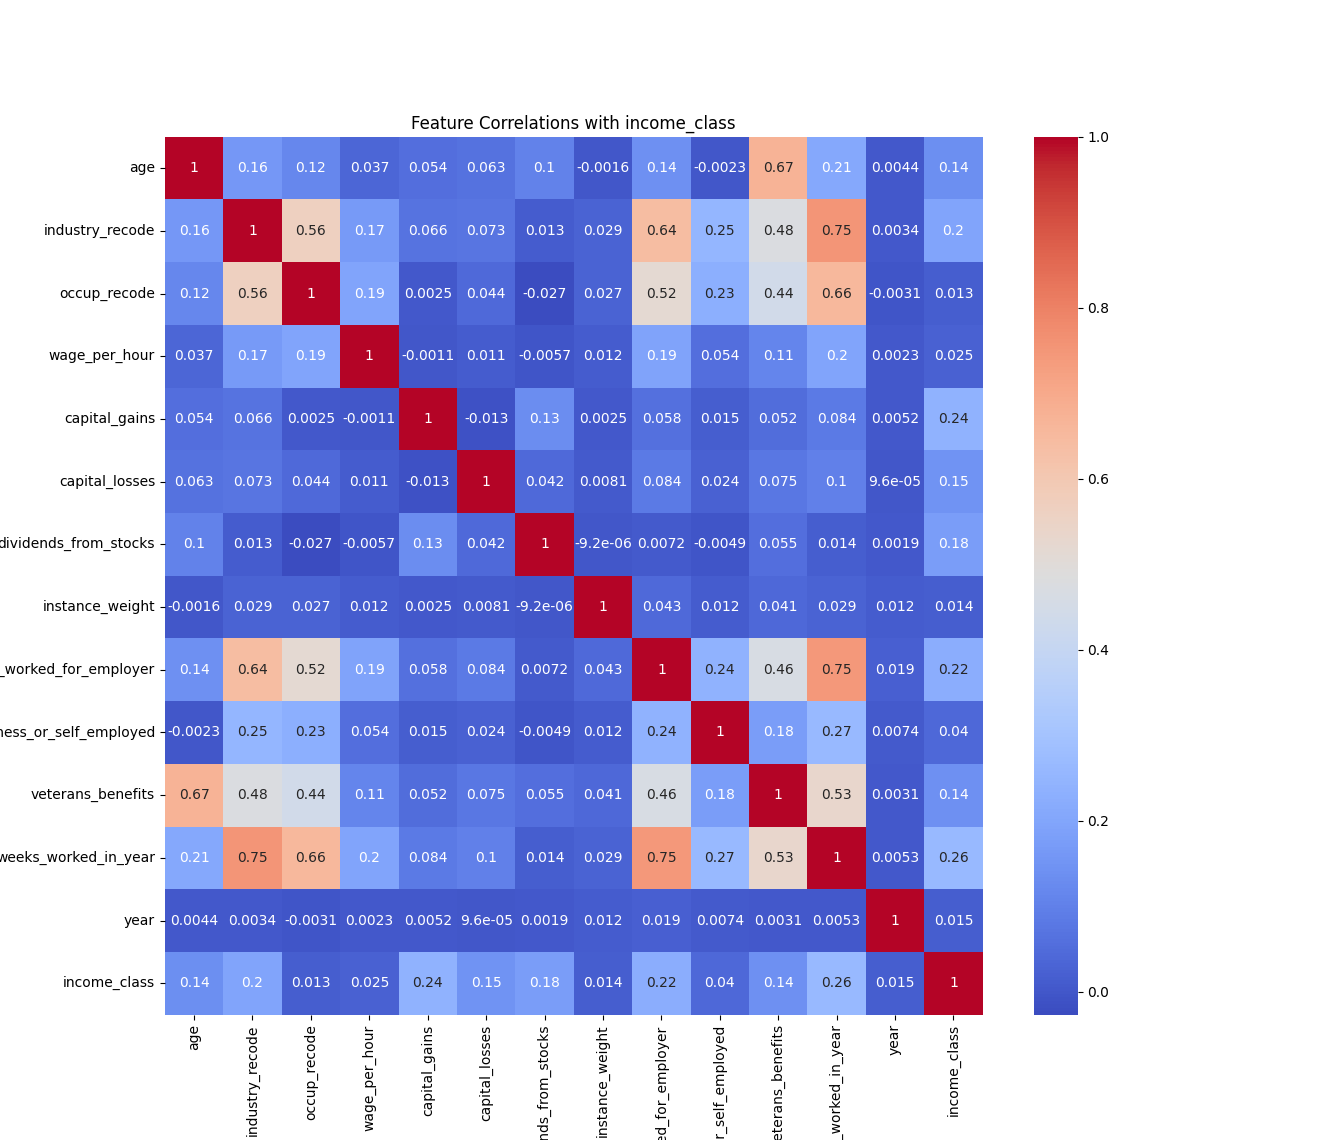
\includegraphics[width=0.8\textwidth]{Figure_2.png}
\end{frame}

\begin{frame}{Feature Importance (Random Forest)}
	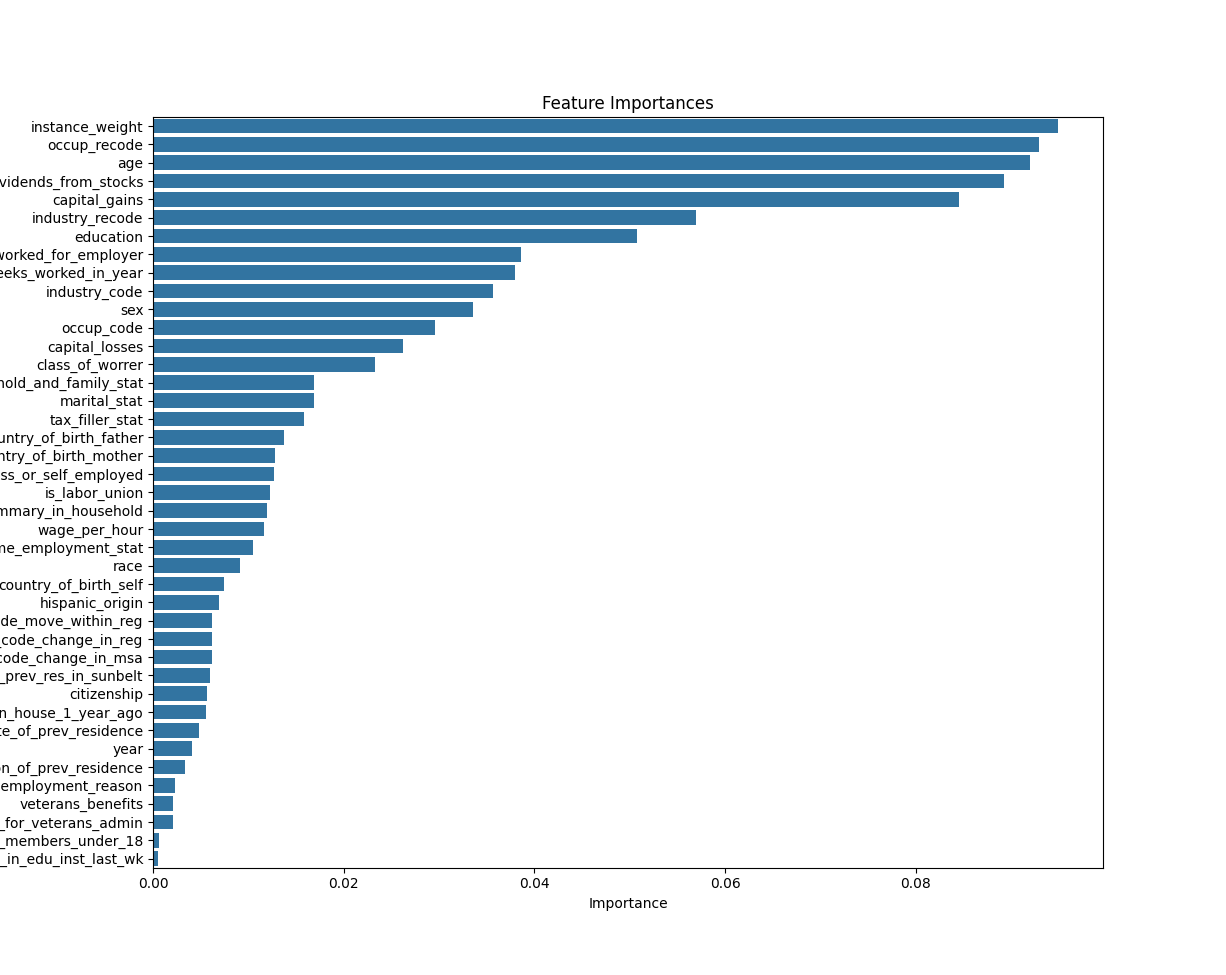
\includegraphics[width=0.9\textwidth]{Figure_1.png}
\end{frame}

\begin{frame}{Models Evaluated}
	\textbf{Algorithms and Performance}
	\begin{enumerate}
		\item \textbf{Logistic Regression}
			\begin{itemize}
				\item \textbf{Strengths}: Simplicity and interpretability.
				\item \textbf{Accuracy}: 95\%, but struggled with recall (28\%) for \texttt{>50K} class.
			\end{itemize}
		\item \textbf{Random Forest}
			\begin{itemize}
				\item \textbf{Strengths}: Non-linear relationships and feature importance.
				\item \textbf{Accuracy}: 95\%, improved recall (39\%) and F1-score for \texttt{>50K}.
			\end{itemize}
		\item \textbf{XGBoost}
			\begin{itemize}
				\item \textbf{Strengths}: Robust handling of imbalanced data.
				\item \textbf{Accuracy}: 95\%, slight decrease in recall (38\%) for \texttt{>50K}.
			\end{itemize}
	\end{enumerate}
\end{frame}

\begin{frame}{Improvements through Hyperparameter Tuning}
	\textbf{Random Forest with GridSearchCV}
	\begin{itemize}
		\item \textbf{Optimized Parameters}:
			\begin{itemize}
				\item \texttt{n\_estimators}: 200
				\item \texttt{max\_depth}: 10
				\item \texttt{min\_samples\_split}: 5
			\end{itemize}
		\item \textbf{Performance}:
			\begin{itemize}
				\item Accuracy: 90\%
				\item Recall for \texttt{>50K}: 76\%
				\item Highlight: Improved balance between precision and recall.
			\end{itemize}
	\end{itemize}
\end{frame}

\begin{frame}{Ensemble Approach}
	\textbf{Custom Soft Voting Ensemble}
	\begin{itemize}
		\item \textbf{Method}:
			\begin{itemize}
				\item Averaged probabilities from Logistic Regression, Random Forest, and XGBoost.
			\end{itemize}
		\item \textbf{Performance}:
			\begin{itemize}
				\item Accuracy: 82\%
				\item Recall for \texttt{>50K}: 92\%
				\item Precision for \texttt{>50K}: 24\%
				\item Tradeoff: Improved recall at the cost of precision.
			\end{itemize}
	\end{itemize}
\end{frame}

\begin{frame}{Summary of Key Takeaways}
	\begin{itemize}
		\item \textbf{Random Forest} was the best model overall, with a balanced tradeoff between precision and recall.
		\item \textbf{Feature Importance} highlighted age, education, and capital gains as key predictors.
		\item \textbf{Custom Ensemble} improved recall significantly but suffered from low precision.
	\end{itemize}
\end{frame}

\begin{frame}{Questions & Discussion}
	\textbf{Let's Collaborate!}
	\begin{itemize}
		\item Questions about methodology?
		\item Suggestions for further improvements?
	\end{itemize}
\end{frame}

\end{document}

